\section{Introduction}
\label{sec:intro}

Please see advice from \href{https://www.cs.columbia.edu/~hgs/etc/intro-style.html}{Prof. Kurose} on how to write a good introduction. 


\textit{A good paper introduction is fairly formulaic. If you follow a simple set of rules, you can write a very good introduction. The following outline can be varied. For example, you can use two paragraphs instead of one, or you can place more emphasis on one aspect of the intro than another. But in all cases, all of the points below need to be covered in an introduction, and in most papers, you don't need to cover anything more in an introduction.}

\textbf{Paragraph 1: Motivation.} \textit{At a high level, what is the problem area you are working in and why is it important? It is important to set the larger context here. Why is the problem of interest and importance to the larger community?}

\textbf{Paragraph 1}: \hl{Video games and streaming have experienced fancier graphics and resolution over the last decades, therefore, it is relevant to ensure if the network traffic classification still works efficiently as it used to. The performed classifications could result as a better allocation of resources allowing us to manage the bandwidth in the most optimal way to avoid wasting it. }

\textbf{Paragraph 2}: \textit{What is the specific problem considered in this paper? This paragraph narrows down the topic area of the paper. In the first paragraph you have established general context and importance. Here you establish specific context and background.}

\textbf{Paragraph 2}: \hl{Nowadays, the fast growth of online activities such as streaming and gaming puts immense demands on the network infrastructure. Traditional approaches to traffic classification cannot stand up to the complexity and diversity of data flows. Our project is aimed at addressing this challenge by leveraging machine learning to differentiate between gaming and music video traffic coming from the same source (youtube) in order to make networks efficient enough to meet the needs of our time.}

\textbf{Paragraph 3}: \textit{"In this paper, we show that ...". This is the key paragraph in the intro - you summarize, in one paragraph, what are the main contributions of your paper given the context you have established in paragraphs 1 and 2. What is the general approach taken? Why are the specific results significant? This paragraph must be really really good. If you can't "sell" your work at a high level in a paragraph in the intro, then you are in trouble. As a reader or reviewer, this is the paragraph that I always look for, and read very carefully.
You should think about how to structure this one or two paragraph summary of what your paper is all about. If there are two or three main results, then you might consider itemizing them with bullets or in test (e.g., "First, ..."). If the results fall broadly into two categories, you can bring out that distinction here. For example, "Our results are both theoretical and applied in nature. (two sentences follow, one each on theory and application)"}

\textbf{Paragraph 3}: \hl{In this paper, we came up with a new approach to traffic classification, which differentiates between gaming and music video, both sourced from YouTube. By using our own dataset and machine learning techniques, our work introduces a classification method by identifying these distinct traffic types. First, instead of training our model on mock data, we consider the real-world traffic data and, through a pipeline performing the key features one by one, such as packet size / frequency, latency, data spikes and flow duration. Our findings reveal that differentiating between gaming and music videos is not just about optimizing network resource allocation, it represents an significant step made toward redesigning and modernizing networks to align with the current era we live in. By addressing this gap, our project lays the groundwork for  smarter and more flexible networking solutions in accordance to the digital era.}

\textbf{Paragraph 4}: \textit{At a high level what are the differences in what you are doing, and what others have done? Keep this at a high level, you can refer to a future section where specific details and differences will be given. But it is important for the reader to know at a high level, what is new about this work compared to other work in the area.}

\textbf{Paragraph 4}: \hl{We came across a related study called Beauty and the Burst, which explores the burstiness of network traffic and how it affects traffic characterization and quality of service. The study offers valuable insights into how bursty behavior impacts network performance across a wide range of applications. However, our approach is different. While Beauty and the Burst focuses on the pattern of traffic at a larger scale, our contribution focuses on the classification of gaming and music video traffic over platforms like YouTube. By using machine learning and a custom dataset specifically designed for this purpose, we restrict ourselves to diving deeper into the unique characteristics of these traffic types and exploring ways to optimize resource allocation more effectively. This focused approach highlights the unique contributions of our work.}

\textbf{Paragraph 5}: \textit{"The remainder of this paper is structured as follows..." Give the reader a roadmap for the rest of the paper. Avoid redundant phrasing, "In Section 2, In section 3, ... In Section 4, ... " etc.}

\textbf{Paragraph 5}: \hl{The rest of this paper is organized as follows. The second section give further insights on the project's purpose and which needs it aims to satisfy explaining how relevant it is in the given context. In the third section we will be describing our approach toward the expected result, breaking it down into different stages such as the data collection process and how we plan to handle them. Throughout the section 4, we will dive deeper into the technical details, focusing on the implementation of our machine learning model specifically. The fifth section will be related to our findings, we will be discussing their relevancy as well as we will compare them to the results expected initially, this section will also be devoted to provide any pertinent graph which is related to our work. Lastly, in Section 6, we summarize the essential conclusions of this work, discuss potential challenges faced, and provide thoughtful suggestions for advancing this research in the future.}

A few general tips:
\begin{itemize}
    \item Don't spend a lot of time into the introduction telling the reader about what you don't do in the paper. Be clear about what you do do, but don't dwell here on what you don't do.
    \item Does each paragraph have a theme sentence that sets the stage for the entire paragraph? Are the sentences and topics in the paragraph all related to each other?
    \item Do all of your tenses match up in a paragraph?
\end{itemize}


Here is a checklist for a good intro from \href{https://docs.google.com/document/d/14g-4txTMwJ4YL61qOcaH6bJWKh59PkI1S-FB1KjeMS4/edit}{Prof. Sherry}: 
\begin{itemize}
    \item Clearly identifies and discusses research problem statement
    \item Motivation and benefits of the research are identified and discussed completely.
    \item Solution/insights of the research are well-articulated.
    \item The problem and/or solution is novel: no one has published something similar before.
    \item ``Teaser'' results provide a useful summary of ``key results''/conclusions of the work.
\end{itemize}


\begin{figure}[t] 
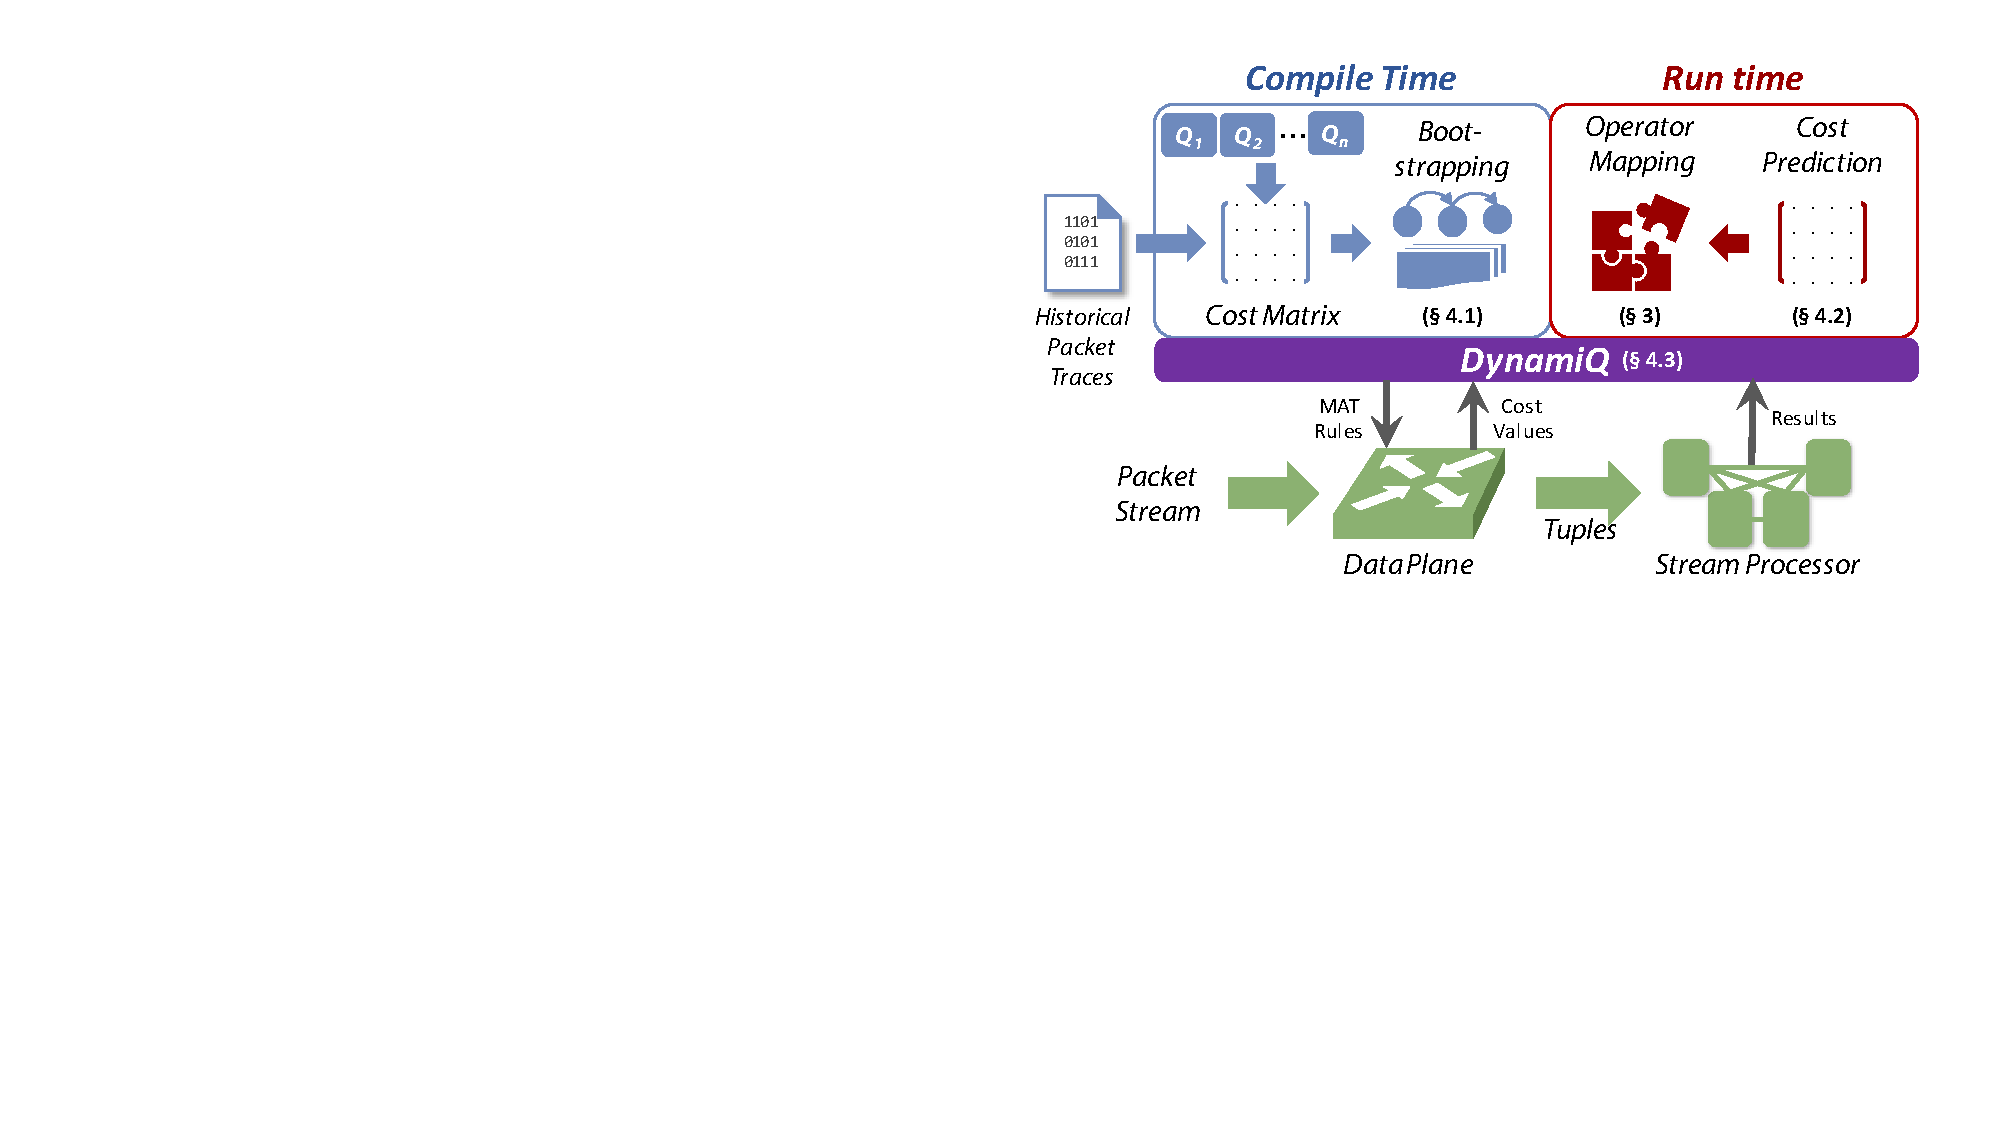
\includegraphics[width=\linewidth]{dynamiq-nutshell.pdf}
\caption{{Sample figure~\cite{sonata}} \label{fig:dynamiq-nutshell}
}
\vspace{-.15in}
\end{figure}
